\section{PLOTR}
\label{sPLOTR}

\hypertarget{sPLOTRhy}{The}
PLOTR module provides a general-purpose plotting capability for
ENDF, PENDF, and GENDF files by generating files that
\hyperlink{sVIEWRhy}{VIEWR} can use
to generate high-quality Postscript plots.  The following kinds of
plots are produced:
\index{PLOTR|textbf}
\index{ENDF}
\index{PENDF}
\index{GENDF}
\index{VIEWR}
\index{plotting}

\begin{itemize}
\begin{singlespace}

\item conventional 2-D plots (for example, cross section {\it vs} energy)
      of ENDF, PENDF, or GENDF data with the normal
      combinations of linear and log scales, automatic or user-specified
      ranges and labels, an optional alternate right-hand axis, and
      with one or two title lines;

\item a set of experimental data by itself or superimposed
      on ENDF, PENDF, or GENDF curves;

\item curves of various patterns,
      labeled with tags and arrows or described in a legend block;

\item data points given with a variety of symbols with error bars (they
      can be identified in a legend block);

\item detailed 3-D perspective plots of File 4 or File 6 angular
      distributions with a choice of a linear or a log axes
      for incident energy and a choice of energy range and viewpoint;

\item selected 2-D plots of File 5 and File 15 emission spectra
      for specified incident
      energies, and selected 2-D emission spectra for given energies
      and particle types for File 6 data;

\item detailed 3-D perspective plots of File 5, 6, or 15  energy
      distributions with a choice of log or linear axes and viewpoint
      (both $E E'\theta$ and $E\theta E'$ laws are supported);

\item 3-D plots of GENDF data; and

\item various 2-D plots for File 7 data, including both symmetric and
      asymmetric $S(\alpha,\beta)$ {\it vs} either $\alpha$ or $\beta$.

\end{singlespace}
\end{itemize}

This section describes the PLOTR module in NJOY2016.0.  As in
NJOY2012 the basic plotting calls have been moved to the
\hyperlink{sVIEWRhy}{VIEWR} module, and the PLOTR module concentrates
exclusively on constructing plots from the data files.  The
coding has been converted into a modular Fortran-90 style.

Methods for generating these types of plots will be given in the
following subsections.  An attempt has been made to keep the input as
simple as possible by moving the less common options to the
right-hand side of each input line so that they can be easily defaulted.
A complete copy of the input instructions will be found in
Section~\ref{ssPLOTR_inp}.  It may be useful to refer to it
occasionally while reading the following sections.

\subsection{Simple 2-D Plots}

The simplest kind of 2-D plot\index{plotting!2-D plots} is for a single
reaction from an ENDF, PENDF, or GENDF file using automatic scales
and default labels.  For example, to plot the total cross section
of carbon from ENDF/B-VII, use the following input (don't type the
line numbers; they are inserted here for reference):

\small
\begin{ccode}

  1.  plotr
  2.  31/
  3.  /
  4.  1/
  5.  '<endf/b-vii carbon'/
  6.  '<t>otal <c>ross <s>ection'/
  7.  4/
  8.  /
  9.  /
 10.  /
 11.  /
 12.  6 20 600 3 1/ tape20 is ENDF/B-VII carbon
 13.  /
 14.  99/
 15.  stop

\end{ccode}
\normalsize

The data to be plotted are selected in line 12 using the normal
MAT, MF, MT notation of ENDF.  The ``slash'' at the end of the
line hides several defaults, the first of which is the temperature,
which defaults to 0K.  The ``4'' in line 7 selects log-log axes
(a number of other options are defaulted here also).  Lines 8
through 11 are blank, resulting in the choice of automatically
defined ranges and default labels.  Two title lines are given
on lines 5 and 6.  Note the use of special shift characters to
change between lowercase and uppercase.  The file on tape31
should be sent through\hyperlink{sVIEWRhy}{VIEWR}
to generate the Postscript plot.  The
result is shown in Fig.~\ref{def2d}.

\begin{figure}[thb]\centering
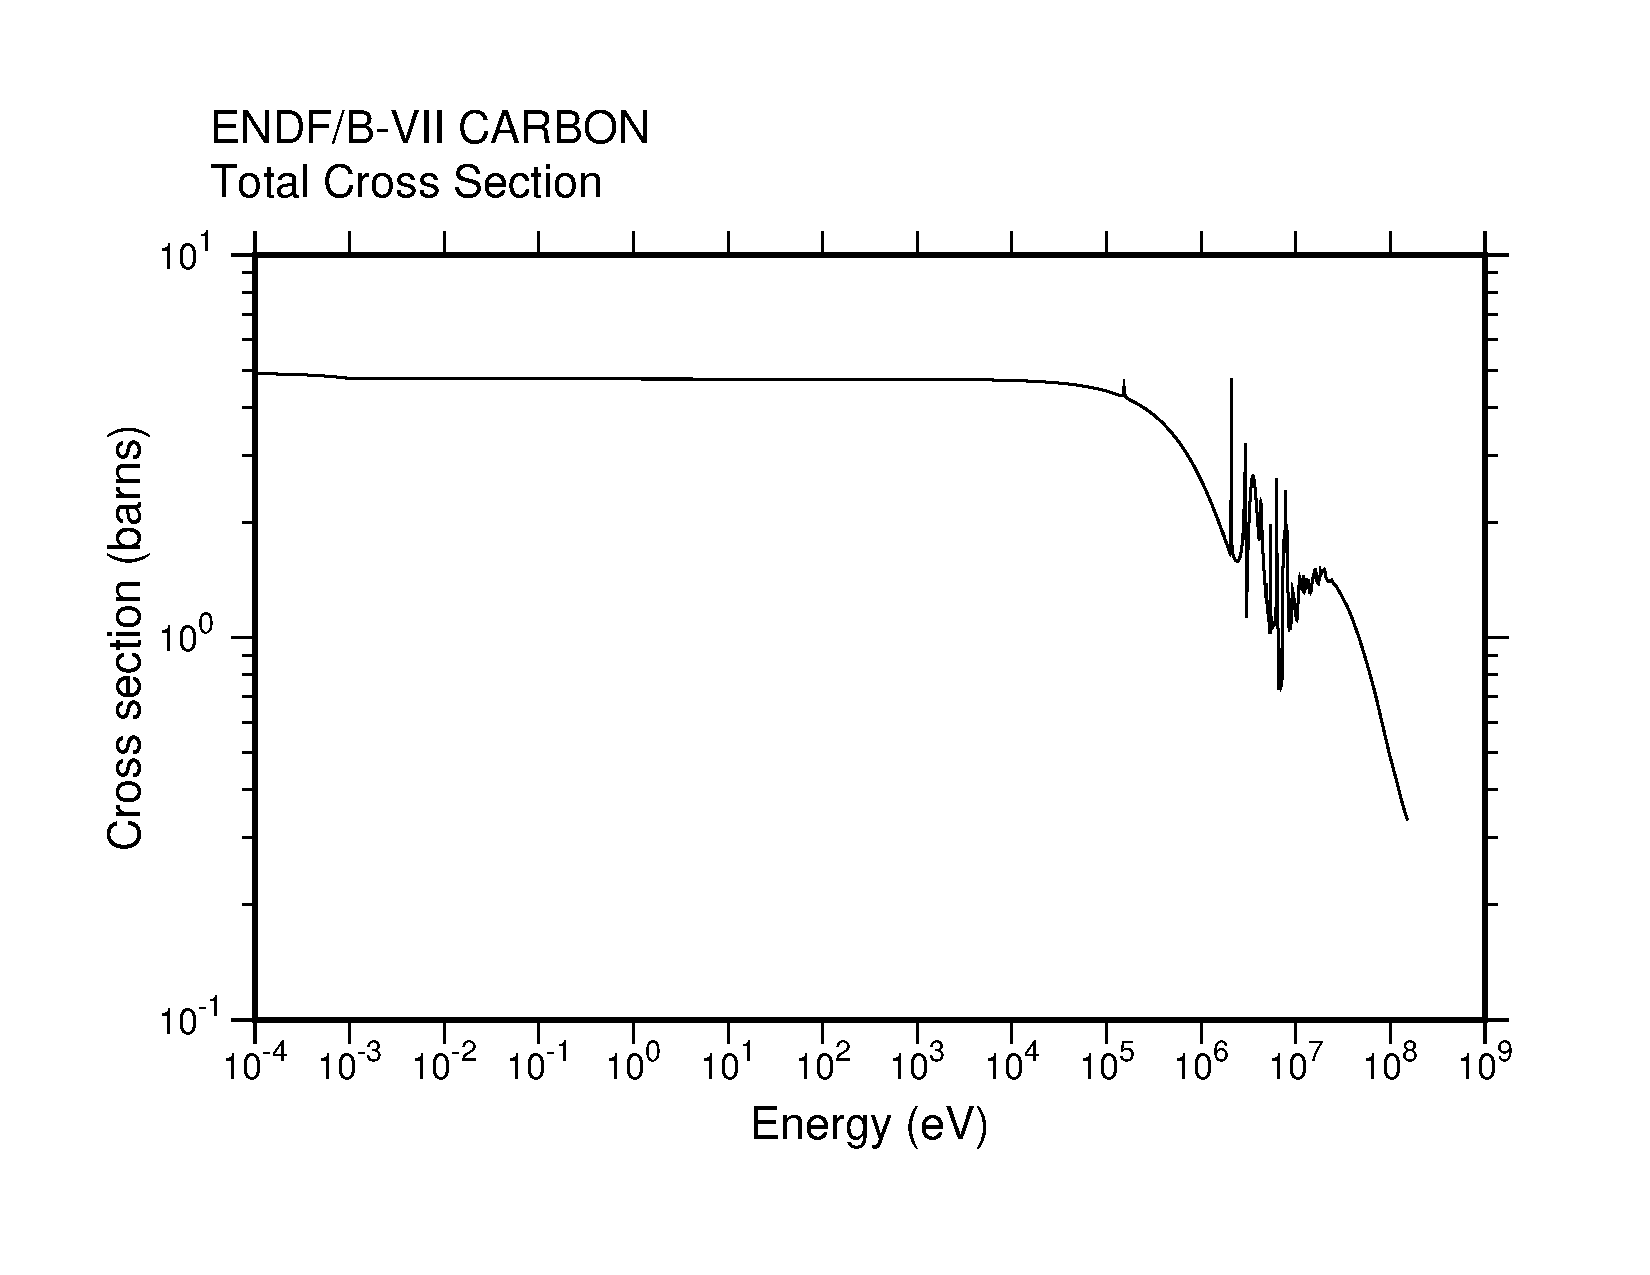
\includegraphics[keepaspectratio, height=3.5in, angle=0]{figs/plotr1ack}
\caption[Sample 2-D plot with default axes]{Simple 2-D plot of the
 total cross section of ENDF/B-VII carbon using automatic log-log axes.}
\label{def2d}
\end{figure}

In many cases, the default scales will give reasonable plots.
However, in this case, the low-energy portion of the plot is
approximately constant. It makes sense to change the lower limit of
the $x$ axis in order to expand the amount of detail shown at higher
energies.  A slight change in the lower limit of the $y$ axis would
also be beneficial.  It is only necessary to change two lines as
follows:

\small
\begin{ccode}

  8.  1e3 2e7/
 10.  .5 10/

\end{ccode}
\normalsize

\noindent
Note that the third parameter on these axes cards should always be
defaulted for log scales.  The results are shown in Fig.~\ref{mod2d}.
This is a better balanced plot.

\begin{figure}[b]\centering
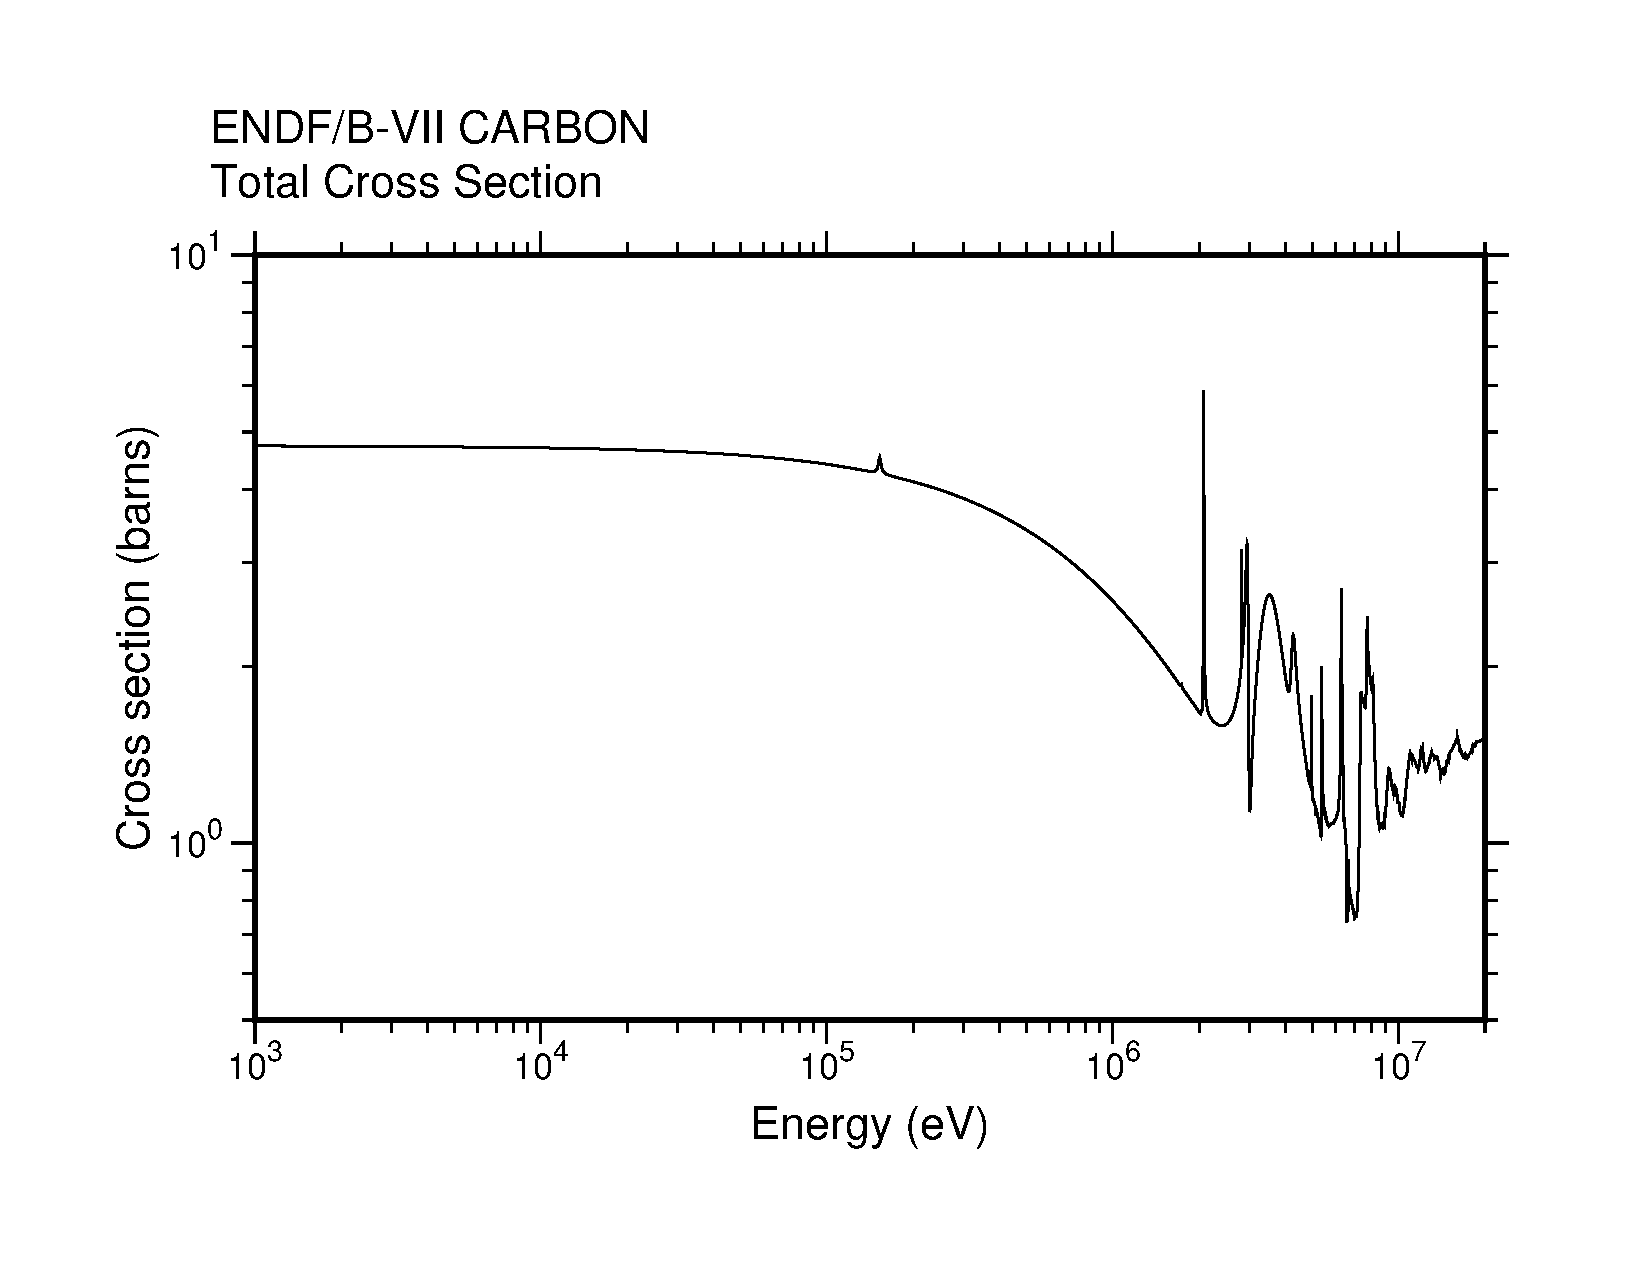
\includegraphics[keepaspectratio, height=3.5in, angle=0]{figs/plotr2ack}
\caption[Sample 2-D plot with modified axes]{Simple 2-D plot of the
 total cross section of ENDF/B-VII carbon using log-log axes with
 user-selected ranges.}
\label{mod2d}
\end{figure}

If the user needs to emphasize the high-energy region, linear scales
are more appropriate.  In addition, some people may prefer a different
font.  The following input gives the results shown in Fig.~\ref{lin2d}.
Note how the new font is specified in line 3.  The linear-linear axes
option is selected in line 7.

\small
\begin{ccode}

  1.  plotr
  2.  31/
  3.  1 1/
  4.  1/
  5.  '<endf/b-vii carbon'/
  6.  '<t>otal <c>ross <s>ection'/
  7.  1/
  8.  /
  9.  /
 10.  /
 11.  /
 12.  6 20 600 3 1/ tape20 is ENDF/B-VII carbon
 13.  /
 14.  99/
 15.  stop

\end{ccode}
\normalsize

\begin{figure}[t]\centering
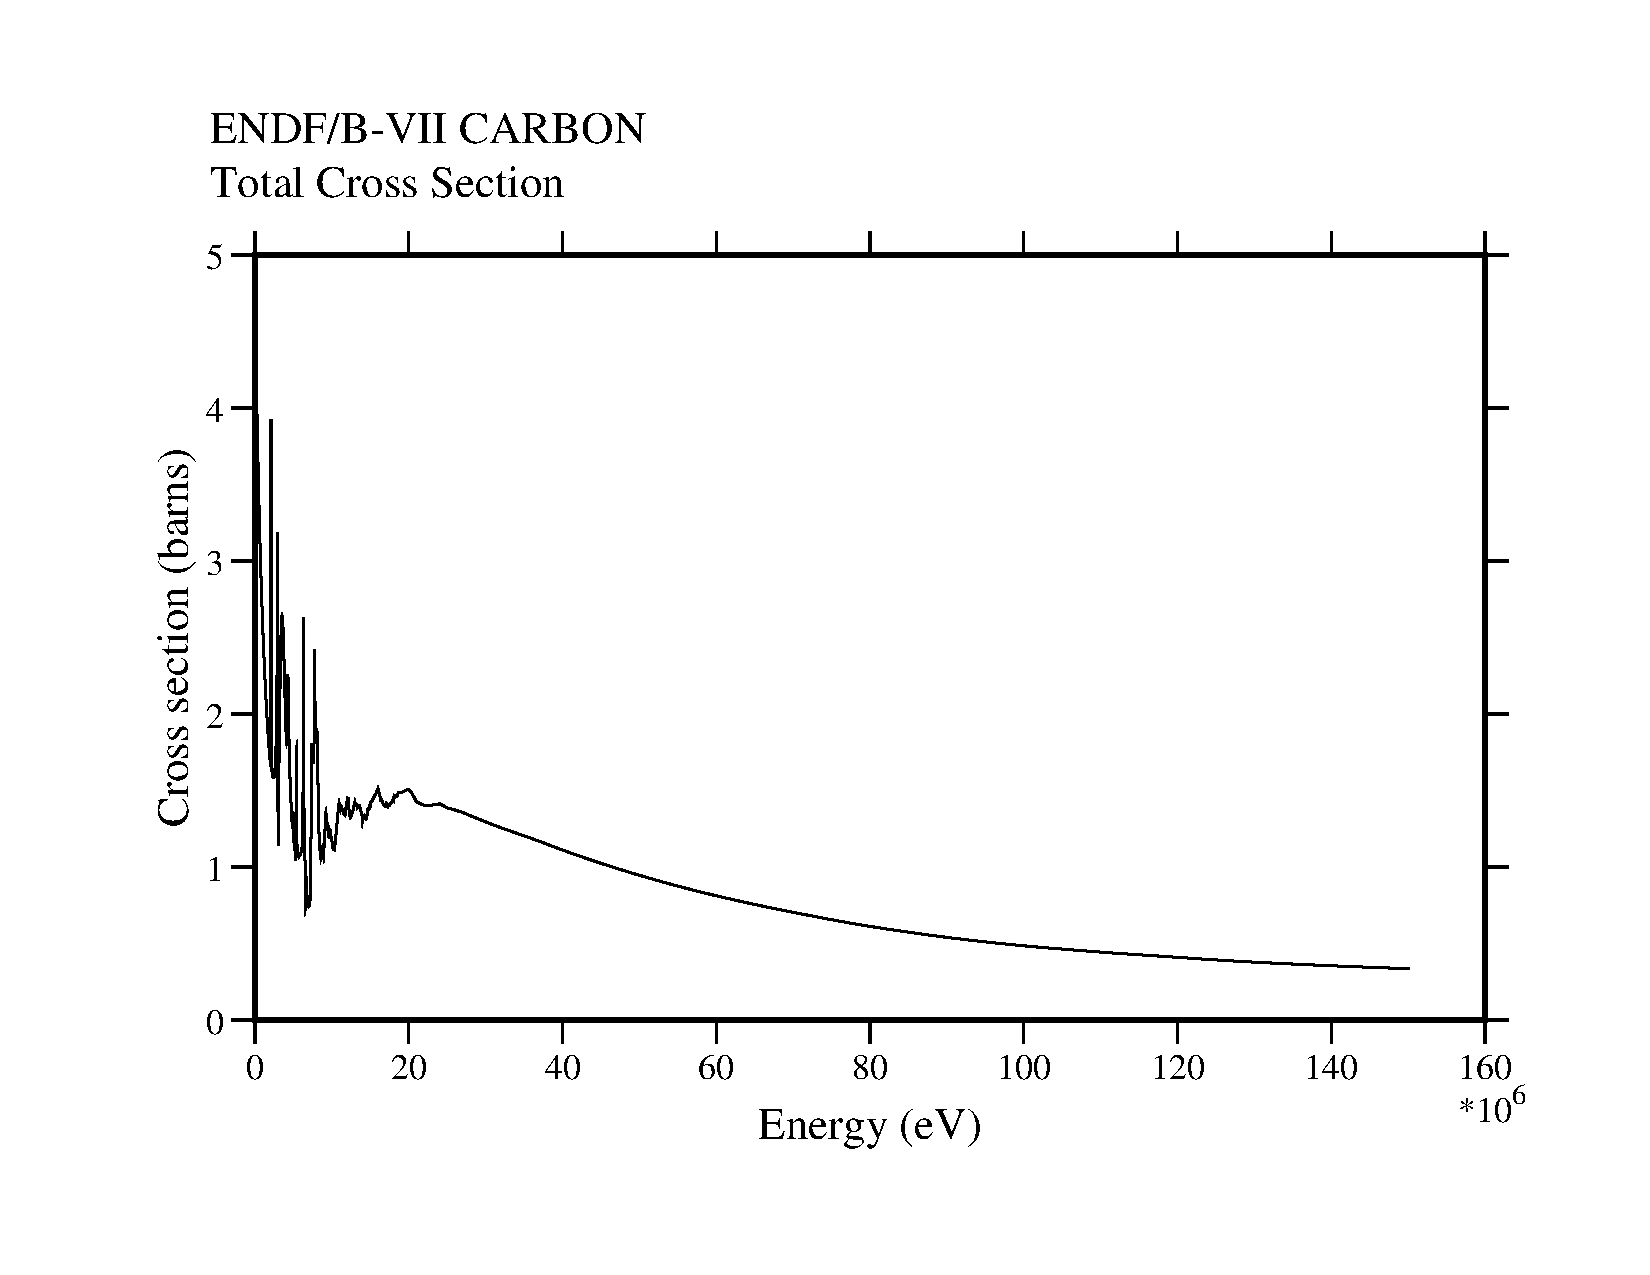
\includegraphics[keepaspectratio, height=3.3in, angle=0]{figs/plotr3ack}
\caption[Sample 2-D plot with linear axes]{Simple 2-D plot of the total
 cross section of ENDF/B-VII.0 carbon using linear axes to emphasize
 the high-energy region and a more elaborate font.}
\label{lin2d}
\end{figure}

\noindent
The limits for the linear $x$ axis in this example could have been
specified by the user with a card of the form

\small
\begin{ccode}

   8.  0 1e7 2e6/

\end{ccode}
\normalsize

\noindent
The general rule for linear axes is either give all three parameters
explicitly, or default all three parameters.  For log axes, either
give the first two parameters and default the third, or default all
three parameters.

Most ENDF or PENDF reactions will have many more energy points
than can be shown on a graph like those in these figures.
Therefore, PLOTR ``thins'' the grid down until there are fewer
than \cword{max} points on the plot (\cword{max} is currently 10 000).
On the other hand, at some energies some ENDF reactions are described
on fairly coarse energy grids using interpolation laws like
``lin-lin'' or ``log-log''.  These representations will look as the
evaluator intended if they are plotted using corresponding scales
(for example, log-log interpolation on log-log scales, or log-lin
interpolation on log-lin scales), but if they were to be plotted
on a different set of axes, the cross sections between the grid
points would be different from those intended.  Therefore, PLOTR
``thickens'' the energy grid by adding additional energy points
between the grid points of the evaluation and computing the cross
section at each of these points from the given interpolation law.
The resulting curves will be faithful to the evaluation, but they
may exhibit unphysical bumps and cusps in certain modes of
presentation.

\subsection{Multicurve and Multigroup Plots}
\label{ssPLOTR_multi}

Several curves can be drawn on each set of axes, and each curve
can be taken from a different data source.  The following input
deck demonstrates how GENDF data can be compared with PENDF data
by overplotting:

\small
\begin{ccode}

   1.  plotr
   2.  31/
   3.  /
   4.  1/
   5.  'ENDF/B-VII #EH.5>241#EXHX>Pu'/
   6.  /
   7.  4 0 2 1 5e3 500/
   8.  .1 2e7/
   9.  /
  10.  1 1e4/
  11.  /
  12.  6 23 9443 3 18 293.6/
  13.  /
  14.  'pointwise fission'/
  15.  2/
  16.  1 24 9443 3 18 293.6 1 1 1/
  17.  0 0 1/
  18.  'multigroup fission'/
  19.  99/
  20.  stop

\end{ccode}
\normalsize

\noindent
The result is shown in Fig.~\ref{pvsm}.  The PENDF data are requested
on Card 12, and the GENDF data are requested on Card 16.  Note the
use of \cword{ivers}=1 to denote GENDF data, and also note the settings
for \cword{nth}, \cword{ntp}, and \cword{nkh} necessary to select the
P$_0$ infinitely dilute cross section for plotting.  The GENDF-format
data are automatically converted into histogram form for plotting.
This example also demonstrates using a ``legend'' block to identify
the two curves.  The position for the legend is given on Card 7.
These values are normally determined by trial and error.  Note also
the presence of a superscript in the title.  The superscript depends
on the \hyperlink{sVIEWRhy}{VIEWR} ``instruction'' mode, which
is described in the \hyperlink{sVIEWRhy}{VIEWR} section of this report.

\begin{figure}[thb]\centering
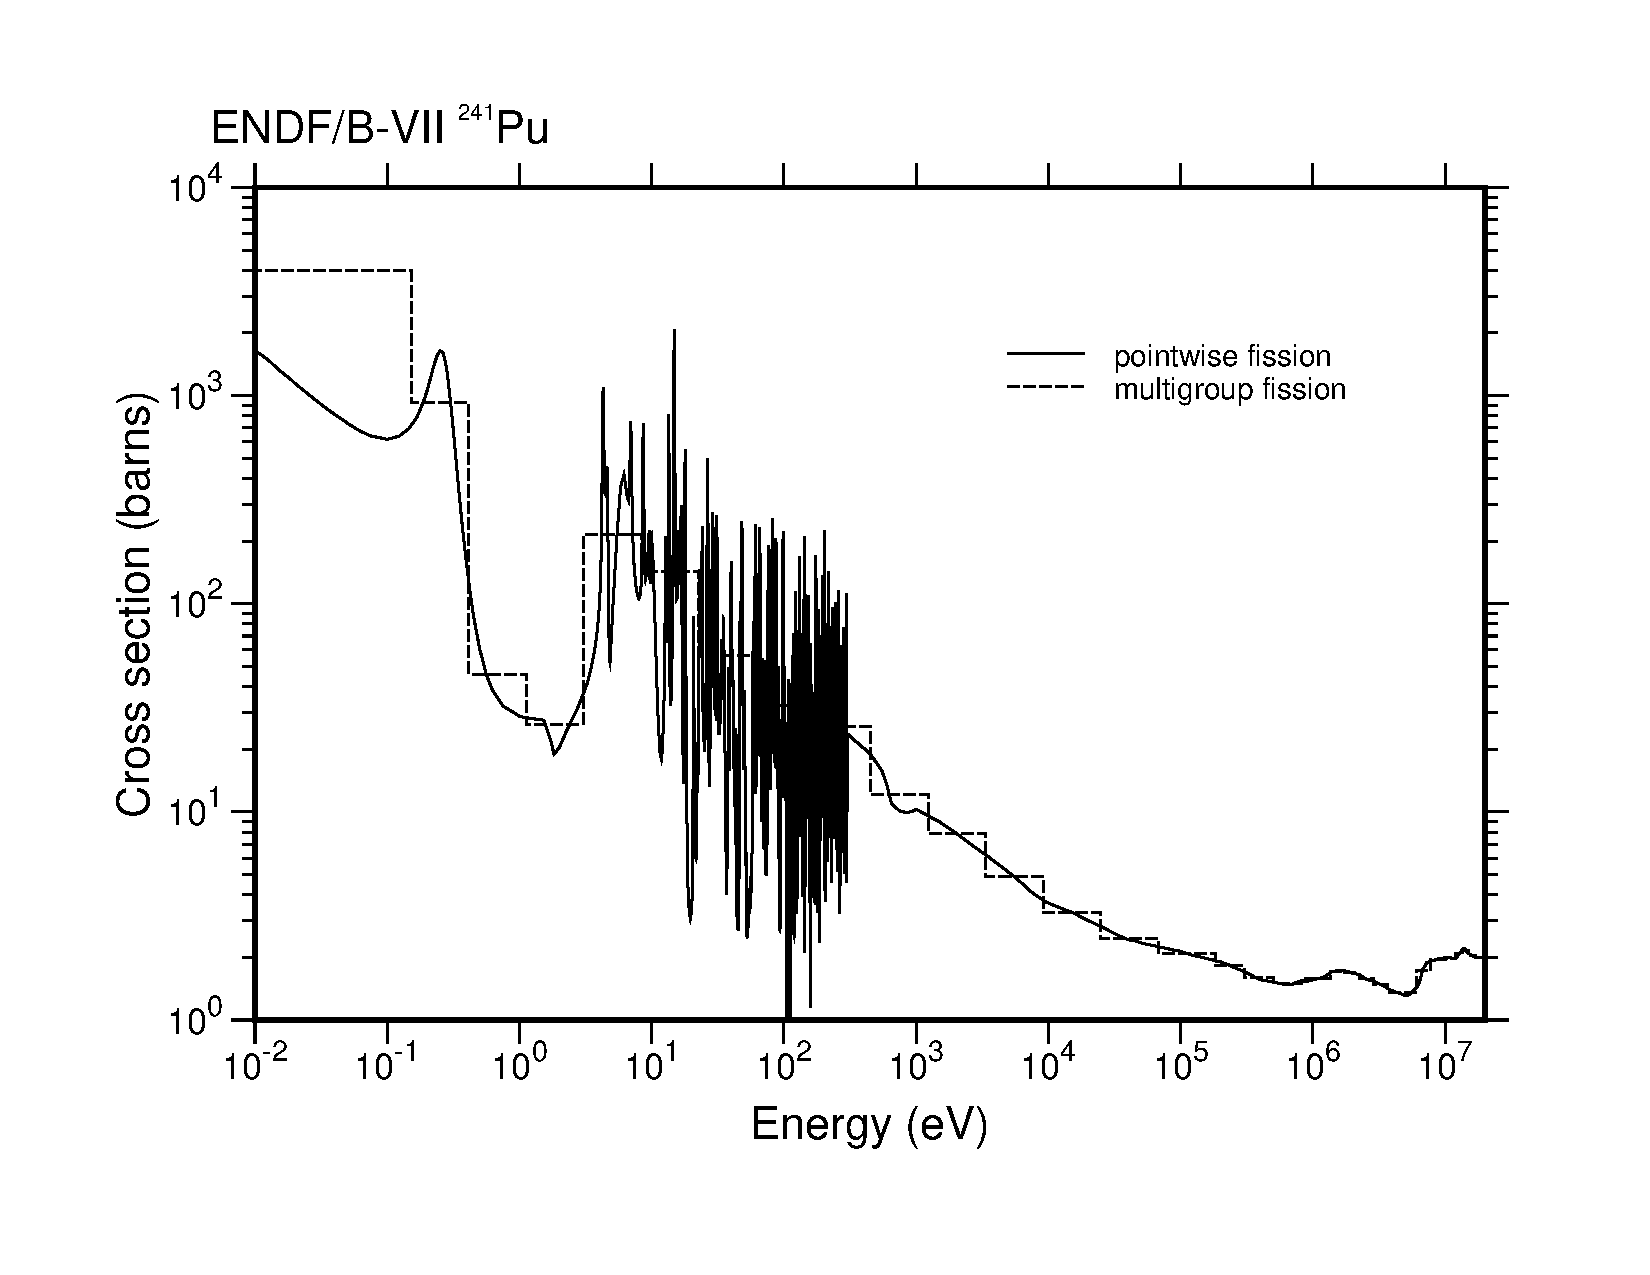
\includegraphics[keepaspectratio, height=3.4in, angle=0]{figs/plotr5ack}
\caption[Sample plot with pointwise and multigroup data]{Comparison of
 the multigroup fission cross section of ENDF/B-VII.0 $^{241}$Pu (dashed curve)
 with the corresponding pointwise cross section from the PENDF tape
 (solid curve).}
\label{pvsm}
\end{figure}

\begin{figure}[thb]\centering
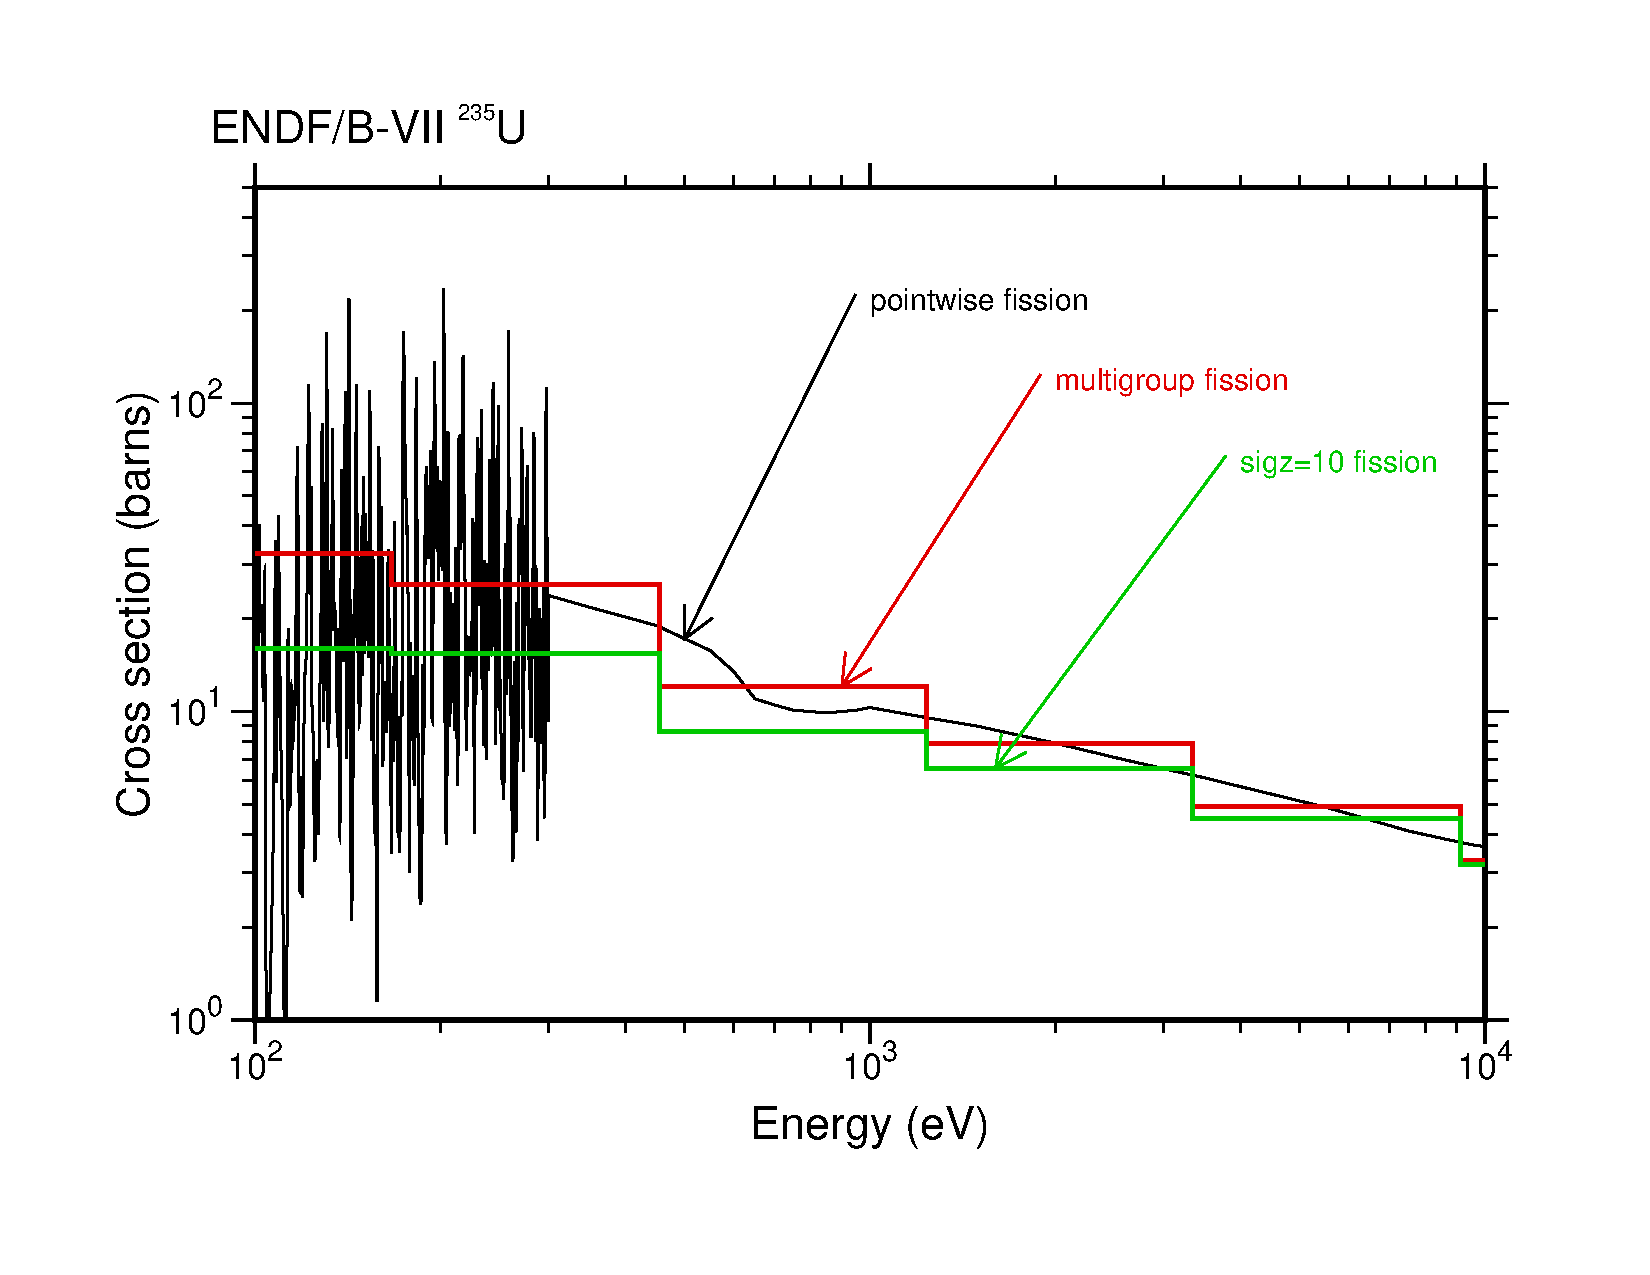
\includegraphics[keepaspectratio, height=3.4in, angle=0]{figs/plotr6ack}
\caption[Sample plot displaying self-shielded cross sections]{Multigroup
 fission cross sections of ENDF/B-VII.0 $^{238}$U for infinite dilution and
 a 10-barn background compared with the corresponding pointwise
 cross section.}
\label{ss}
\end{figure}

As another example of a plot of multigroup data, Fig.~\ref{ss}
shows both infinitely dilute and self-shielded cross sections,
and the plot also compares them with the pointwise cross section.
In order to distinguish better between the different curves,
color and double width are used.  Here are the curve colors
currently allowed:

{
\begin{verbatim}
   curve color (def=black)
     0=black
     1=red
     2=green
     3=blue
     4=magenta
     5=cyan
     6=brown
     7=purple
     8=orange
\end{verbatim}}

In addition, this plot uses ``tags'' and arrows to identify the
different curves.  The position of the tags and the
$x$ location for the arrowhead usually must be determined by
trial and error.  See lines 15, 20 and 25, which give the x and
y coordinates of the tag and x coordinate where the arrow
head meets the curve.  The input for this example follows:

\newpage
\small
\begin{ccode}

  1.  plotr
  2.  31/
  3.  /
  4.  1/
  5.  'ENDF/B-VII #EH.5>235#EXHX>U'/
  6.  /
  7.  4 0 2 2/
  8.  100 10000/
  9.  /
 10.  1 500/
 11.  /
 12.  6 23 9443 3 18 293.6/
 13.  /
 14.  'pointwise fission'/
 15.  1000 200 500/
 16.  2/
 17.  1 24 9228 3 18 293.6 1 1 1/
 18.  0 0 1 2/
 19.  'multigroup fission'/
 20.  2000 110 900/
 21.  3/
 22.  1 24 9228 3 18 293.6 1 3 1/
 23.  0 0 2 2/
 24.  ']#S+LH.5>0#LXHX>=10 fission'/
 25.  4000 60 1600/
 26.  99/
 27.  stop

\end{ccode}
\normalsize

\noindent
This example requires 293.6K PENDF data for $^{235}$U on the
input file \cword{tape23} and 293.6K multigroup data for $\sigma_0=\infty$,
$\sigma_0=500$ barns, and $\sigma_0=10$ barns on \cword{tape24}.
These tapes can be generated with the following NJOY input deck:

\small
\begin{ccode}

   1.  reconr
   2.  20 21/ tape20 is U-235
   3.  /
   4.  9228/
   5.  .1/
   6.  0/
   7.  broadr
   8.  20 21 22/
   9.  9228 1/
  10.  .1/
  11.  293.6/
  12.  0/
  13.  unresr
  14.  20 22 23/
  15.  9228 1 3 1/
  16.  293.6/
  17.  1e10 500 10/
  18.  0/
  19.  groupr
  20.  20 23 0 24/
  21.  9228 3 0 3 1 1 3 1/
  22.  /
  23.  293.6/
  24.  1e10 500 10/
  25.  3 1/
  26.  3 18/
  27.  3 102/
  28.  0/
  29.  0/
  30.  stop

\end{ccode}
\normalsize

\subsection{Right-Hand Axes}
\label{ssPLOTR_righthand}

PLOTR supports the capability to have different ordinate scales
on the left and right sides of a graph.  One place where this
can be used is plotting a data curve and the ratio of another
data curve to the first curve.  An example of this is shown
in Fig.~\ref{rhax}.  The input file used to make this plot is
shown below.  The \hyperlink{sRECONRhy}{RECONR} module
is run twice to make zero $^\circ$K
PENDF files for plotting.  Note the minus signs on lines
28 and 35 --- this selects the right-hand scale for those sections
of the input.  In line 36, the value of \cword{nth} of 3
request the ratio calculation, and the additional input card
in line 37 is read to access the second material for the ratio.

\begin{figure}[b]\centering
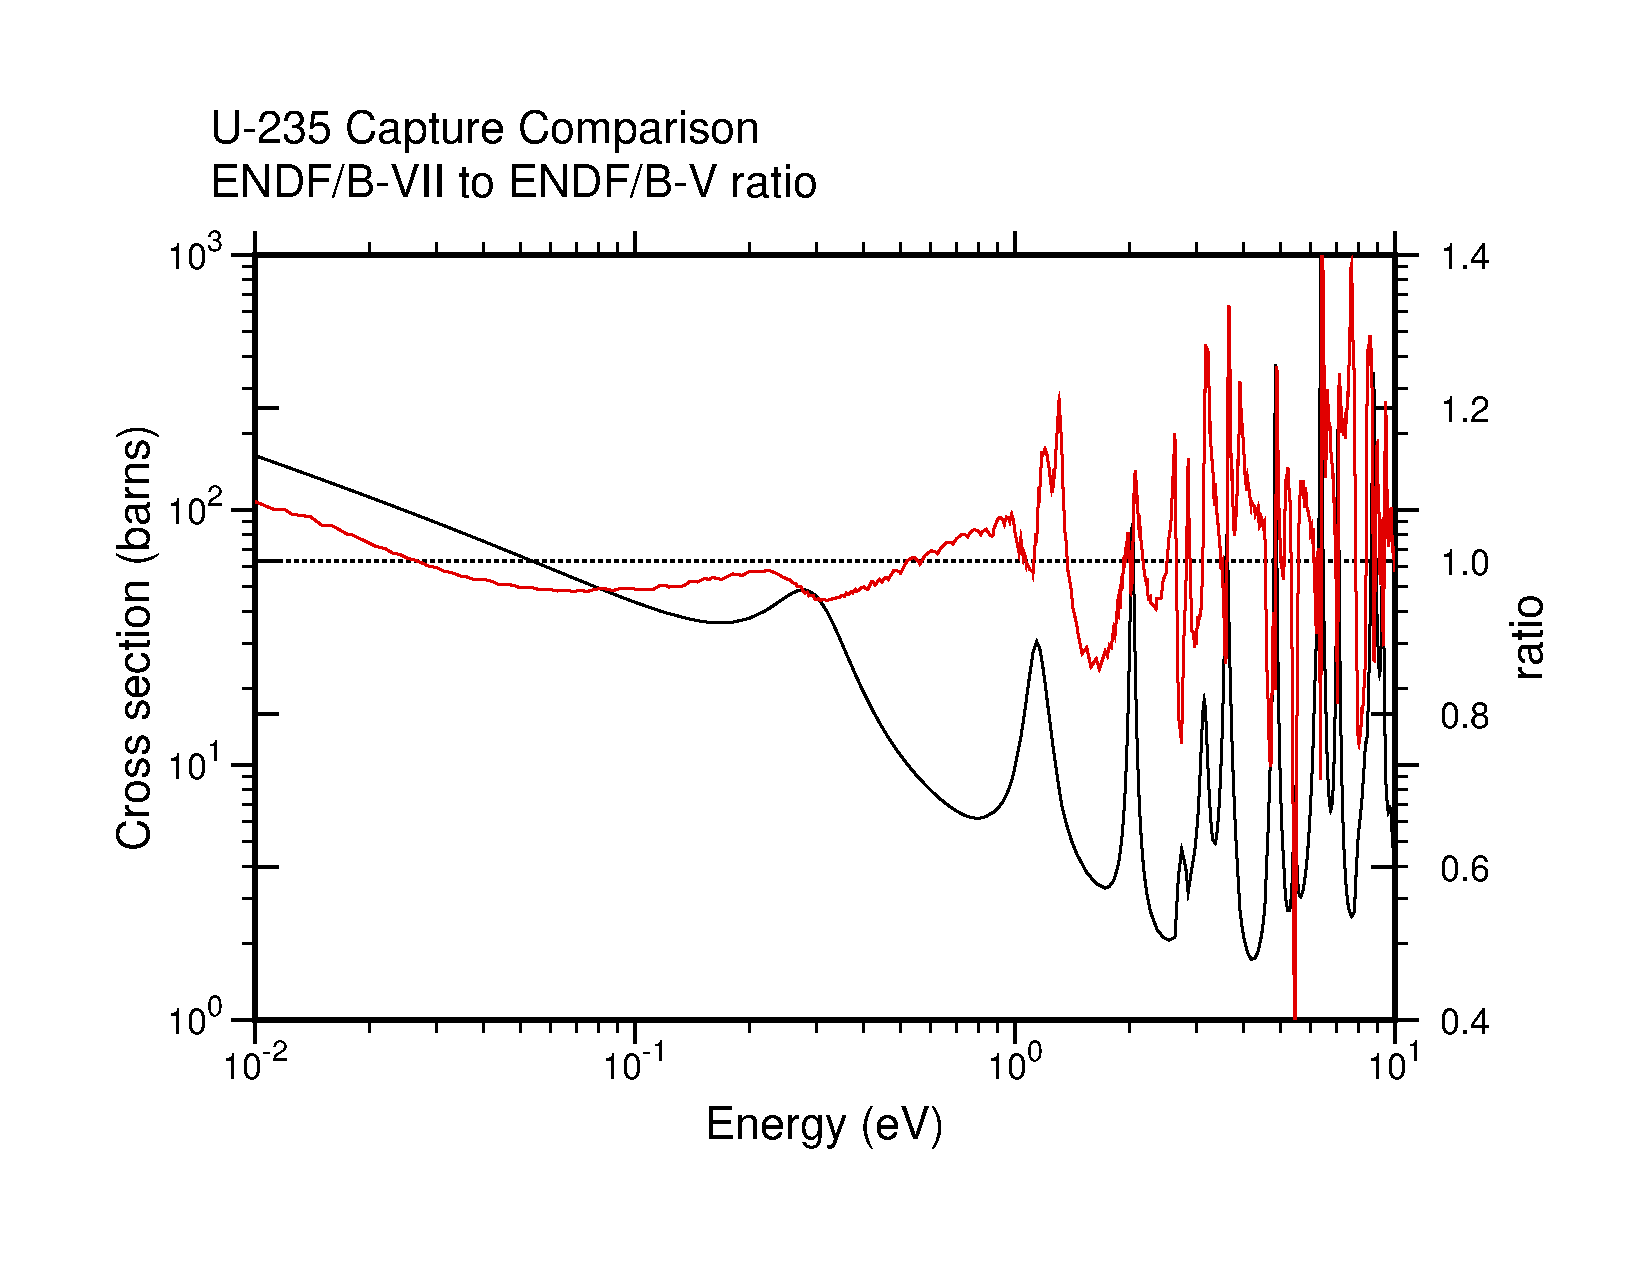
\includegraphics[keepaspectratio, height=3.6in,angle=0]{figs/plotr6aack}
\caption[Sample plot with left- and right-hand axes defined]{Using a right-hand
 axis to plot the ratio of the ENDF/B-VII.0 capture cross section for $^{235}$U
 to the ENDF/B-V value.  The black curve is the ENDF/B-V cross section, and
 the red curve is the ratio (right-hand axis).}
\label{rhax}
\end{figure}

\small
\begin{ccode}
  1. reconr
  2. 20 22/ tape20 ENDF/B-V U-235
  3. /
  4. 1395/
  5. .02/
  6. 0/
  7. reconr
  8. 21 23/ tape20 ENDF/B-VII U-235
  9. /
 10. 9228/
 11. .02/
 12. 0/
 13. plotr
 14. 31/
 15. /
 16. 1/
 17. 'U-235 Capture Comparison'/
 18. 'ENDF/B-VII to ENDF/B-V ratio'/
 19. 4 1/
 20. 1e-2 10/
 21. /
 22. /
 23. /
 24. 0.4 1.4 .2/
 25. 'ratio'/
 26. 5 22 1395 3 102/ tape20 is carbon from V
 27. /
 28. -2/
 29. 0/
 20. 0 0 4/
 31. 0/
 32. 1e-2 1./
 33. 10. 1./
 34. /
 35. -3/
 36. 5 22 1395 3 102 0. 1 3/ tape20 is carbon from V
 37. 6 23 9228 3 102 0./
 38. 0 0 0 1/
 39. 99/
 40. stop
\end{ccode}
\normalsize


\subsection{Plotting Input Data}
\label{ssPLOTR_inp_data}

PLOTR allows the user to insert data directly into the input deck.
\index{experimental data}
The main use of this is to superimpose experimental data over curves
obtained from ENDF, PENDF or GENDF tapes, but reading data directly
from the input deck can also be used to add precalculated curves or
eye guides to plots, or to add special features such as vertical lines
to separate regions on plots.  Experimental data points can be plotted
with a variety of symbols, and $x$ and/or $y$ error bars can be included
if desired.  The error bars can be either symmetric or asymmetric.  For
experimental data, the curves and various sets of data points are
normally identified using a legend block.  The following input produces
a typical example of this type of plot:

\small
\begin{ccode}

   1.  plotr
   2.  31/
   3.  /
   4.  1/
   5.  'ENDF/B-VII CARBON'/
   6.  '(n,]a>) with fake data'/
   7.  1 0 2 1 1.3e7 .25/
   8.  6e6 18e6/
   9.  /
  10.  /
  11.  /
  12.  6 20 600 3 107/
  13.  /
  14.  'ENDF/B-VII MAT 600'/
  15.  2/
  16.  0/
  17.  -1 0/
  18.  '<s>mith & <s>mith 1914'/
  19.  0/
  20.  1.1e7 .08 .05 .05/
  21.  1.2e7 .10 .05 .05/
  22.  1.3e7 .09 .04 .04/
  23.  1.4e7 .08 .03 .03/
  24.  /
  25.  3/
  26.  0/
  27.  -1 2/
  28.  'Black & Blue 2008'/
  29.  0/
  30.  1.15e7 .07 .02 0. .2e6 0./
  31.  1.25e7 .11 .02 0. .2e6 0./
  32.  1.35e7 .08 .015 0. .2e6 0./
  33.  1.45e7 .075 .01 0. .2e6 0./
  34.  /
  35.  99/
  36.  stop

\end{ccode}
\normalsize

The results are shown in Fig.~\ref{data}. The error bars for both of
these simulated data sets are symmetric, as indicated explicitly in
Cards 20 through 23, or by the zeroes in Cards 30 through 33.  They
can also be asymmetric if the lower and upper (or right and left)
values are nonzero and different.

\begin{figure}[b]\centering
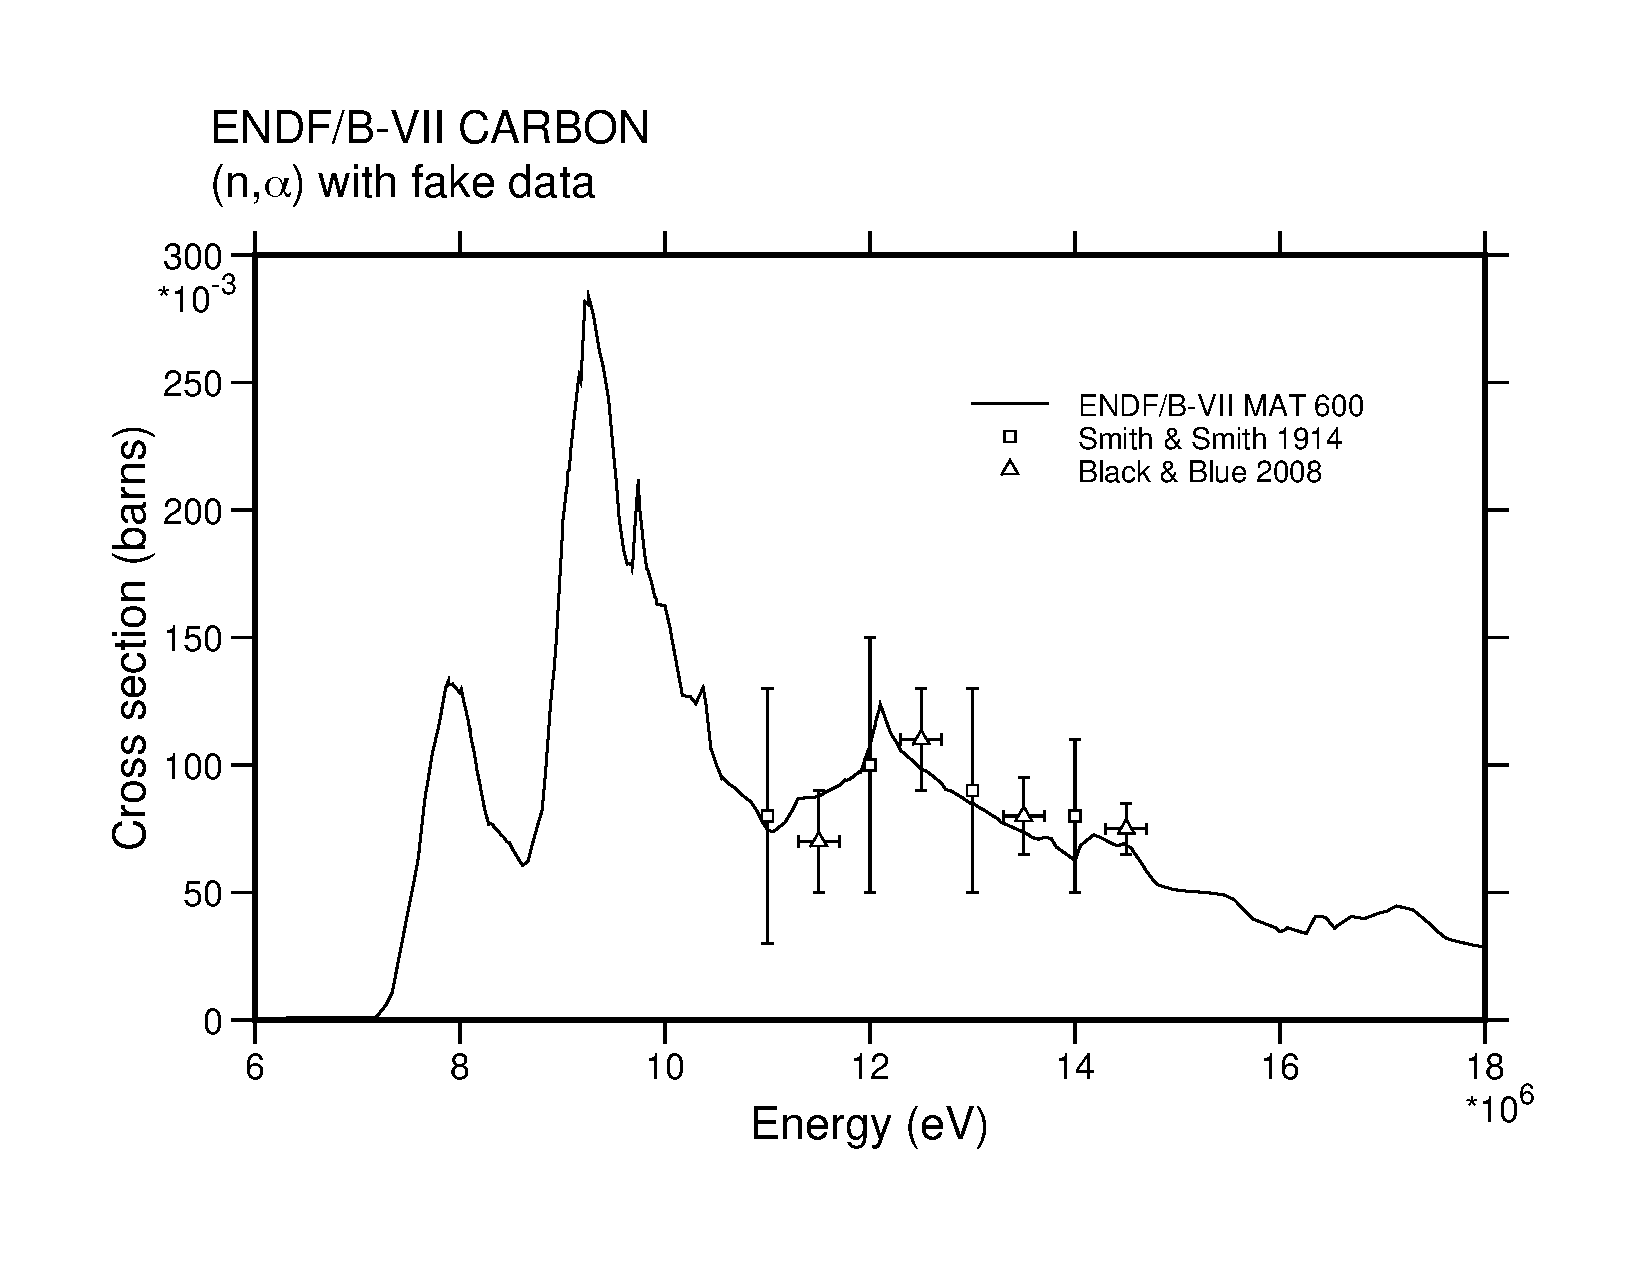
\includegraphics[keepaspectratio, height=3.6in, angle=0]{figs/plotr7ack}
\caption[Sample plot with user data]{Carbon (n,$\alpha$) cross section
 compared with two sets of simulated experimental data represented
 with two types of error bars.}
\label{data}
\end{figure}

\subsection{Three-D Plots of Angular Distributions}
\label{ssPLOTR_3D_angdist}

ENDF angular distribution data, whether given in File 4 or File 6,
\index{plotting!3-D plots}
can be very bulky.  Therefore, it is useful to present them in the
form of a perspective plot showing a family of angular distribution
curves for each value of incident particle energy.  An input
deck to make such a perspective plot follows:

\small
\begin{ccode}
   1.  plotr
   2.  31/
   3.  /
   4.  1/
   5.  'ENDF/B-V CARBON'/
   6.  'Elastic MF4'/
   7.  -1 2/
   8.  /
   9.  /
  10.  1e6 5e6 1e6/
  11.  /
  12.  /
  13.  /
  14.  5 20 1306 4 2/
  15.  /
  16.  99/
  17.  stop
\end{ccode}
\normalsize

\noindent
Fig.~\ref{angd} shows the result using a linear axis for incident
energy.  This axis is the $y$ axis, and its range has been limited to
expand a particular part of the distribution.  A linear scale emphasizes
the high-energy region.

\begin{figure}[b]\centering
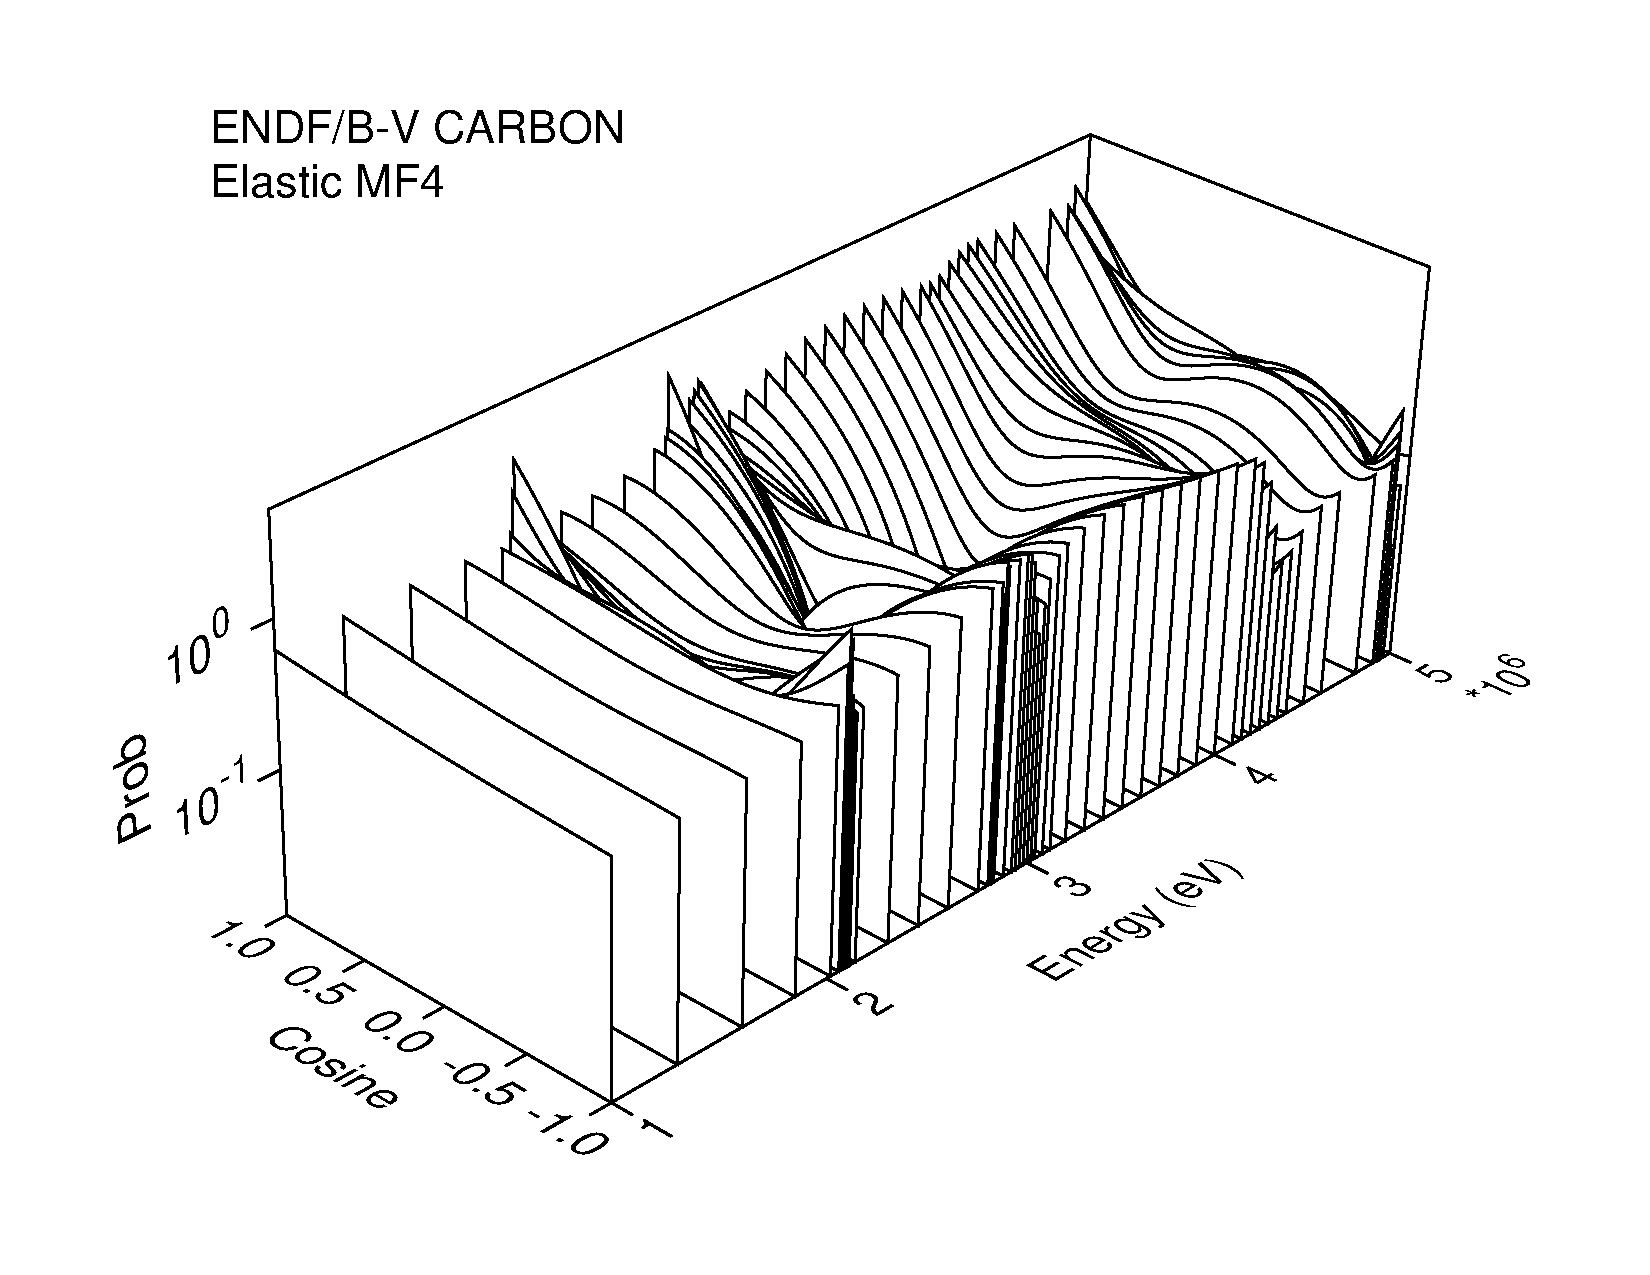
\includegraphics[keepaspectratio, height=3.25in, angle=0]{figs/plotr8ack}
\caption[Sample 3-D plot of angular distribution data]{Perspective view
 of carbon elastic scattering angular distribution.}
\label{angd}
\end{figure}


\subsection{Three-D Plots of Energy Distributions}
\label{ssPLOTR_3D_energydist}

Three-D perspective plots are also useful for energy distributions.
For the ENDF-5 and earlier formats, neutron secondary-energy
distributions are given in File 5.  The following input deck
shows how to request a 3-D plot for File 5:

\small
\begin{ccode}

   1.  plotr
   2.  31/
   3.  /
   4.  1/
   5.  'ENDF/B-V Li-6'/
   6.  '(n,2n)]a neutron distribution'/
   7.  -1 2 1/
   8.  /
   9.  /
  10.  4e6 20e6 2e6/
  11.  /
  12.  5 20 1303 5 24/
  13.  /
  14.  99/
  15.  stop

\end{ccode}
\normalsize

\noindent
Grids lines have been requested in Card 7.  The result is shown in
Fig.~\ref{enerd}.  Similar methods can be used to plot photon emission
distributions from File 15.

The new ENDF-6 format also provides for giving distributions
\index{ENDF!ENDF format!ENDF-6 format}
for other emitted particles, such a protons, alphas, photons,
and even recoil nuclei.  This complicates the task of selecting
which distribution is to be extracted from File 6.
The user must specify the index for the particular outgoing
particle to be considered (see \cword{nkh}). Line 12 might become,
for example,

\small
\begin{ccode}

  12.  6 20 2437 103 0. 0 0 1/

\end{ccode}
\normalsize

\noindent
which would request a plot of the proton distribution for the
(n,p) reaction of $^{54}$Cr from ENDF/B-VI.

\begin{figure}[thb]\centering
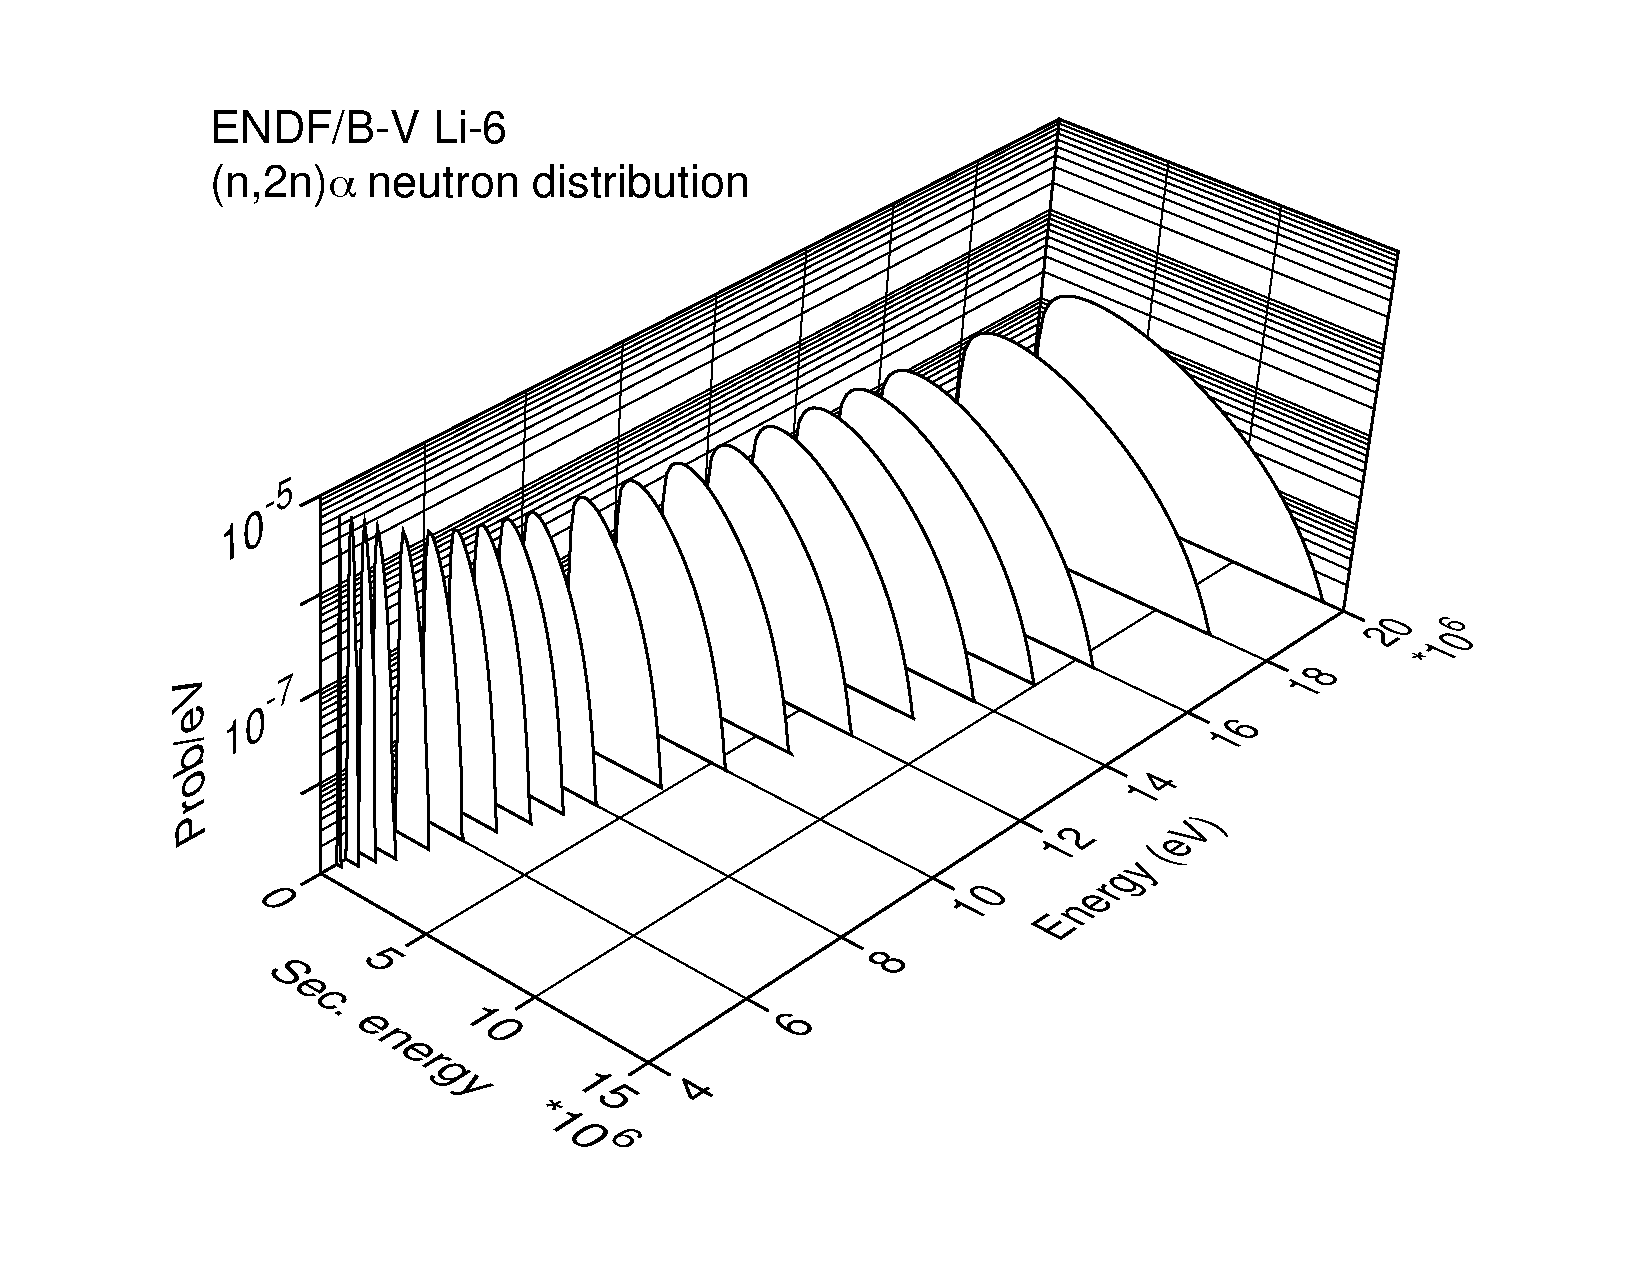
\includegraphics[keepaspectratio, height=3.6in, angle=0]{figs/plotr9ack}
\caption[Sample 3-D plot of neutron secondary-energy distribution data]
{Perspective plot of $^{6}$Li (n,2n)$\alpha$ neutron secondary-energy
 distributions.}
\label{enerd}
\end{figure}

For some evaluations, File 6 uses Law 7, where the energy-angle
\index{File 6}
distribution is represented as $E{\rightarrow}E'$ distributions
for several emission cosines $\mu$.  In these cases, the \cword{ntp}
parameter may be used to select one of the emission angles, and
the 3-D plot shows the distribution for that angle.

\subsection{Two-D Spectra Plots from Files 5 and 6}
\label{ssPLOTR_2D_mf5_mf6}

It is difficult to see real detail on 3-D plots, and the emission
spectra cannot be compared with measurements.  Therefore, PLOTR has
the capability to extract the spectrum for a particular particle
and incident energy.  The following input deck shows how several
such spectra can be plotted on one graph.

\small
\begin{ccode}

   1.  plotr
   2.  31/
   3.  /
   4.  1/
   5.  'ENDF/B-V Li-6'/
   6.  '(n,2n)]a >neutron spectra vs <E>'/
   7.  4 0 2 2/
   8.  10. 2.e7/
   9.  /
  10.  1e-11 1e-6/
  11.  '<c>ross <s>ection (barns/e<V>)'/
  12.  5 20 1303 5 24 0. 12/
  13.  /
  14.  '10 <m>e<v>'/
  15.  1e3 2e-11 1e2/
  16.  2/
  17.  5 20 1303 5 24 0. 16/
  18.  /
  19.  '14 <m>e<v>'/
  20.  1e4 2e-10 2e3/
  21.  3/
  22.  5 20 1303 5 24 0. 20/
  23.  /
  24.  '20 <m>e<v>'/
  25.  1e5 2e-9 4e4/
  26.  99/
  27.  stop

\end{ccode}
\normalsize

\noindent
The results are shown in Fig.~\ref{spec}.  ``Tags'' are used to
distinguish between the different incident energy values.

\begin{figure}[t]\centering
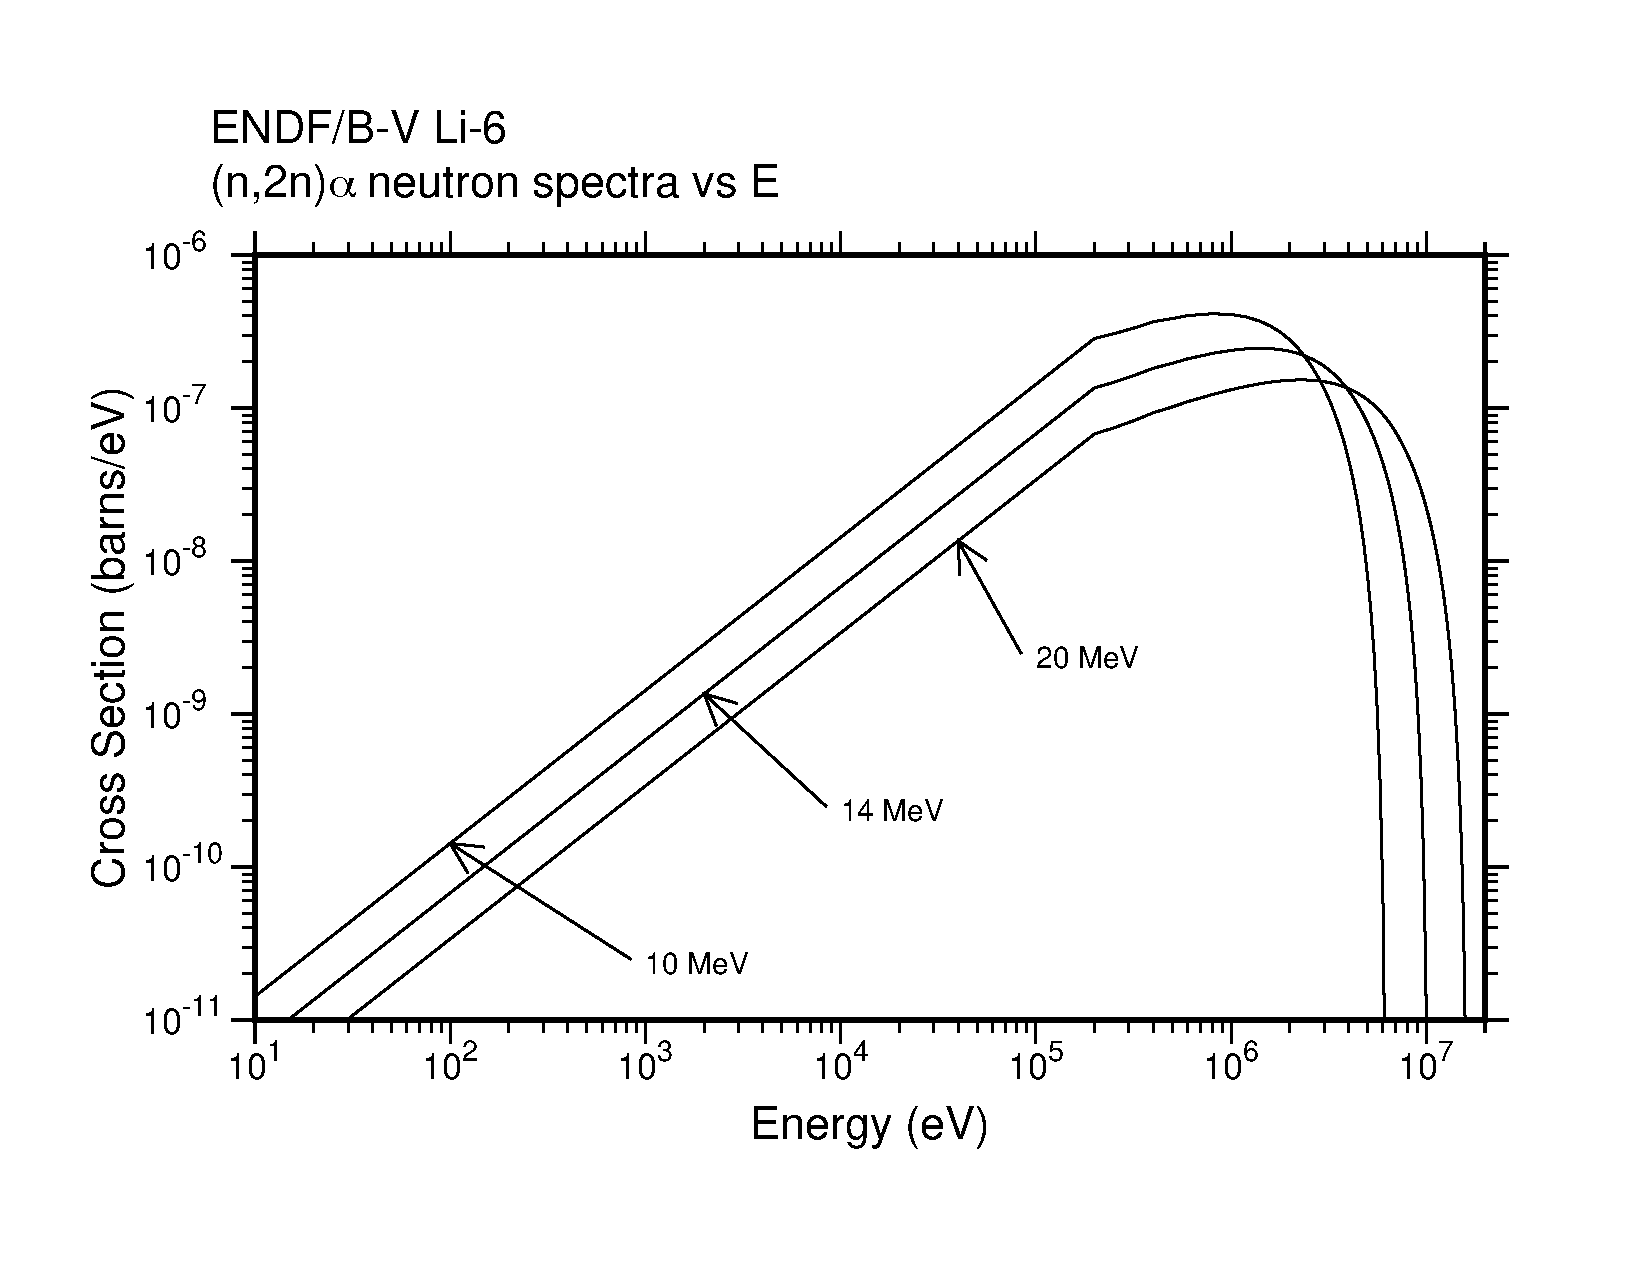
\includegraphics[keepaspectratio, height=3.6in, angle=0]{figs/plotr10ack}
\caption[Sample 2-D plot of neutron secondary-energy distribution data]
{Two-D plot of selected secondary neutron spectra for the
 $^{6}$Li (n,2n)$\alpha$ reaction.}
\label{spec}
\end{figure}

The method used for selecting which curve is to be plotted
is awkward in the current version of PLOTR.  The user must give
the index number of the incident energy desired (like the value
12 in line 12 of this example).

When an ENDF-6 format File 6 is available, emission spectra
\index{File 6}
will normally be given for several emitted particles, photons,
and recoil nuclei.  In addition, angular data may be given for
various $E{\rightarrow}E'$ transfers using several different
representations.  This complicates the task of selecting which
curve is to be extracted from File 6.  For Law 1 data, the
user must specify the particular outgoing particle to be
considered (see \cword{nkh}), the index for the incident energy
desired (see \cword{nth}), and the dependent variable to plot (see
\cword{ntp}).  The result depends on the representation used.  In
every case, \cword{ntp}=1 gives the cross section versus $E'$, but
for Legendre polynomials, \cword{ntp}=2 gives the P$_1$ component
versus $E'$, and for Kalbach-Mann, \cword{ntp}=2 gives the
preequilibrium ratio versus $E'$.  For Law 7, \cword{ntp} specifies the
emission angle.  The graph will show a spectrum versus $E'$ for
the specified angle, specified incident energy $E$, and specified
particle.


\subsection{Input Instructions}
\label{ssPLOTR_inp}
\index{PLOTR!PLOTR input}
\index{input!PLOTR}

\small
\begin{ccode}

   !---input--------------------------------------------------------
   !
   !  card 0
   !     nplt          unit for output plot commands
   !     nplt0         unit for input plot commands
   !                     default=0=none
   !                     output plot commands are appended
   !                     to the input plot commands, if any.
   !  card 1
   !     lori          page orientation (def=1)
   !                    0  portrait (7.5x10in)
   !                    1  landscape (10x7.5in)
   !     istyle        character style (def=2)
   !                     1 = roman
   !                     2 = swiss
   !     size          character size option
   !                     pos = height in page units
   !                     neg = height as fraction of subplot size
   !                     (default=0.30)
   !     ipcol         page color (def=white)
   !                    0=white
   !                    1=navajo white
   !                    2=blanched almond
   !                    3=antique white
   !                    4=very pale yellow
   !                    5=very pale rose
   !                    6=very pale green
   !                    7=very pale blue
   !
   ! -----repeat cards 2 through 13 for each curve-----
   !
   !  card 2
   !     iplot         plot index
   !                     99 = terminate plotting job
   !                      1 = new axes, new page
   !                     -1 = new axes, existing page
   !                      n = nth additional plot on existing axes
   !                     -n = start a new set of curves using
   !                          the alternate y axis
   !                     default = 1
   !     iwcol         window color (def=white)
   !                    color list same as for ipcol above
   !     factx         factor for energies (default=1.)
   !     facty         factor for cross-sections (default=1.)
   !     xll,yll       lower-left corner of plot area
   !     ww,wh,wr      window width, height, and rotation angle
   !                   (plot area defaults to one plot per page)
   !
   ! -----cards 3 thru 7 for iplot = 1 or -1 only-----
   !
   !  card 3
   !     t1            first line of title
   !                   60 characters allowed.
   !                   default=none
   !
   !  card 3a
   !     t2            second line of title
   !                   60 characters allowed.
   !                   default=none
   !
   !  card 4
   !     itype         type for primary axes
   !                     1 = linear x - linear y
   !                     2 = linear x - log y
   !                     3 = log x - linear y
   !                     4 = log x - log y
   !                     set negative for 3d axes
   !                     default=4
   !     jtype         type for alternate y axis or z axis
   !                     0 = none
   !                     1 = linear
   !                     2 = log
   !                     default=0
   !     igrid         grid and tic mark control
   !                     0 = no grid lines or tic marks
   !                     1 = grid lines
   !                     2 = tic marks on outside
   !                     3 = tic marks on inside
   !                     default=2
   !     ileg          option to write a legend.
   !                     0 = none
   !                     1 = write a legend block with upper left
   !                         corner at xtag,ytag (see below)
   !                     2 = use tag labels on each curve with
   !                         a vector from the tag to the curve
   !                     default=0
   !     xtag          x coordinate of upper left corner
   !                   of legend block
   !     ytag          y coord of upper left corner
   !                   default=upper left corner of plot
   !
   !  card 5
   !     el            lowest energy to be plotted
   !     eh            highest energy to be plotted
   !     xstep         x axis step
   !                   default = automatic scales
   !                   (default all 3, or none)
   !                   (the actual value of xstep is
   !                       ignored for log scales)
   !
   !  card 5a
   !     xlabl         label for x axis
   !                   60 characters allowed.
   !                    default="energy (ev)"
   !
   !  card 6
   !     yl            lowest value of y axis.
   !     yh            highest value of y axis.
   !     ystep         step for y ayis (linear scales only)
   !                   default = automatic scales
   !                   (default all 3, or none)
   !                   (the actual value of ystep is
   !                       ignored for log scales)
   !
   !  card 6a
   !     ylabl         label for y axis
   !                   60 characters allowed.
   !                    default="cross section (barns)"
   !
   !  card 7   (jtype.gt.0 only)
   !     rbot          lowest value of secondary y axis or z axis
   !     rtop          highest value of secondary y axis or z axis
   !     rstep         step for secondary y axis or z axis
   !                   default for last three = automatic
   !
   !  card 7a  (jtype.gt.0 only)
   !     rl            label for alternate y axis or z axis
   !                   60 characters allowed.
   !                   default=blank
   !
   !  -----cards 8 thru 9 are always given-----
   !
   !  card 8
   !     iverf         version of endf tape
   !                     set to zero for data on input file
   !                       and ignore rest of parameters on card
   !                     set to 1 for gendf data
   !     nin           input tape
   !                   can change for every curve if desired.
   !     matd          desired material
   !     mfd           desired file
   !     mtd           desired section
   !                    mtd=0 means loop over all reactions in mfd
   !                    (usually one page per mt, but for mf=3,
   !                    resonance reactions may have several pages)
   !     temper        temperature for endf data (degK, default=0.)
   !     nth,ntp,nkh   see below (defaults=1)
   !
   !       special meanings for nth,ntp,nkh for file 3 or 5 data
   !            nth   number of subsection to plot
   !              (works for isomer prod, delayed n, etc.)
   !            ntp   not used
   !            nkh   not used
   !
   !       special meanings for nth for file 4 Legendre data
   !            nth   index for Legendre coefficient (p1, p2, ...)
   !
   !       special meanings for nth,ntp,nkh for file 6 data
   !            nth   index for  incident energy
   !            ntp   number of dep. variable in cyle to plot
   !                  (or angle number for law 7)
   !            nkh   number of outgoing particle to plot
   !
   !       special meanings for nth,ntp,nkh for gendf mf=3 data
   !            nth=0 for flux per unit lethargy
   !            nth=1 for cross section (default)
   !            ntp=1 for infinite dilution (default)
   !            ntp=2 for next lowest sigma-zero values, etc.
   !            nkh=1 for p0 weighting (default)
   !            nkh=2 for p1 weighting (total only)
   !
   !       special meaning for nth for gendf mf=6 data
   !            nth=1 plot 2-d spectrum for group 1
   !            nth=2 plot 2-d spectrum for group 2
   !              etc.
   !        no special flags are needed for mf=6 3d plots
   !
   !      special meanings for nth and ntp for mf7 plots
   !           nth is index for indep. variable (alpha or beta)
   !           ntp=1 selects alpha as indep. variable (default)
   !           ntp=2 selects beta as indep. variable
   !           nkh=1 selects normal s(alpha,beta)
   !           nkh=2 selects script s(alpha,-beta)
   !           nkh=3 selects script s(alpha,beta)
   !
   ! -----cards 9 and 10 for 2d plots only-----
   !
   !  card 9
   !     icon          symbol and connection option
   !                     0 = points connected, no symbols
   !                    -i = points not connected, symbol at every
   !                         ith point
   !                     i = points connected, symbol at every ith
   !                         points
   !                     default=0
   !     isym          no. of symbol to be used
   !                     0 = square
   !                     1 = octagon
   !                     2 = triangle
   !                     3 = cross
   !                     4 = ex
   !                     5 = diamond
   !                     6 = inverted triangle
   !                     7 = exed square
   !                     8 = crossed ex
   !                     9 = crossed diamond
   !                     10 = crossed octagon
   !                     11 = double triangle
   !                     12 = crossed square
   !                     13 = exed octagon
   !                     14 = triangle and square
   !                     15 = filled circle
   !                     16 = open circle
   !                     17 = open square
   !                     18 = filled square
   !                     default=0
   !     idash         type of line to plot
   !                     0 = solid
   !                     1 = dashed
   !                     2 = chain dash
   !                     3 = chain dot
   !                     4 = dot
   !                     default=0
   !     iccol         curve color (def=black)
   !                     0=black
   !                     1=red
   !                     2=green
   !                     3=blue
   !                     4=magenta
   !                     5=cyan
   !                     6=brown
   !                     7=purple
   !                     8=orange
   !     ithick        thickness of curve (def=1)
   !                     0 = invisible (for shaded areas)
   !     ishade        shade pattern
   !                     0 = none
   !                     1 to 10 = 10\% to 100\% gray
   !                     11 to 20 = 45 deg right hatching
   !                     21 to 30 = 45 deg left hatching
   !                     31 to 40 = 45 deg cross hatching
   !                     41 to 50 = shades of green
   !                     51 to 60 = shades of red
   !                     61 to 70 = shades of brown
   !                     71 to 80 = shades of blue
   !                     default=0
   !
   !  card 10  ---ileg.ne.0 only---
   !     aleg          title for curve tag or legend block
   !                   60 characters allowed.
   !                   default=blank
   !
   !  card 10a  ---ileg.eq.2 only---
   !     xtag          x position of tag title
   !     ytag          y position of tag title
   !     xpoint        x coordinate of vector point
   !                    (.le.0 to omit vector)
   !
   ! -----card 11 for 3d plots only-----
   !
   !  card 11
   !     xv,yv,zv      abs. coords of view point
   !                   defaults=15.,-15.,15.
   !     x3,y3,z3      abs. sides of work box volume
   !                   defaults=2.5,6.5,2.5
   !
   !         set x3 or y3 negative to flip the order of the
   !         axis on that side of the work box.
   !
   !  -----cards 12 thru 13 for iverf = 0 only-----
   !
   !  card 12
   !     nform          format code for input data
   !                    0 = free format input with
   !                    optional x and y error bars
   !
   !  card 13   ---nform = 0 only---
   !     xdata          dependent value
   !                    terminate with empty card (/)
   !     ydata          independent value
   !     yerr1          lower y error limit
   !                    no y error bar if zero
   !     yerr2          upper y error limit
   !                    if zero, equals yerr1
   !     xerr1          x left error limit
   !                    no x error bar if zero
   !     xerr2          x right error limit
   !                    if zero, equals xerr1
   !
   ! all curves contain at least 10 points per decade (see delta).
   ! code can plot curves containing fewer than 2000 points (see
   ! max) without thinning.  curves with more points are thinned
   ! based on a minimum spacing determined from max and the
   ! length of the x axis.
   !
   !--------------------------------------------------------------------
\end{ccode}
\normalsize

\subsection{Coding Details}
\label{ssPLOTR_details}

Subroutine \cword{plotr}\index{plotr@{\ty plotr}}
is the only public call in the module
\cword{plotm}\index{modules!plotm@{\ty plotm}}.
It starts by setting up the default paper size,
margins, working box, and view point.  It then reads in the first
two input cards to define the unit for Postscript output and the
parameters for the graphics page, such as orientation, font style,
font size, and page color. The routine can then start the main
loop over plots, subplots, and curves (see statement number 110).
The next card is read, which gives the value of \cword{iplot}.
If \cword{iplot}=99, the job is complete and the code exits
through statement number 700 by writing an end ``99'' on the plot
file and closing the open units.

The next step is to start reading the user's input.  For each input
line, the defaults are set and the standard Fortran READ* method is
used to read the input.  Once all the input parameters have been read,
the code branches to different regions for different data types.

For ENDF and PENDF data, PLOTR reads the first part of File 1
and searches for the desired temperature.  It then uses
\cword{findf}\index{findf@{\ty findf}}
to locate the desired material and reaction.  Note that there
is an option for an automatic reaction loop that enters at
statement number 320.  When \cword{mtd}=0, \cword{plotr} automatically
loops over all the MT numbers that it finds in the current file.
For 2-D plots, it is necessary to extract the desired $x$ and $y$ values
out of a TAB1 or a LIST record.  It is fairly tricky finding
this record because of the large number of possible formats
in Files 3, 5, 6, 7, and 15.  Some improvements are
needed here to allow PLOTR to construct angular distributions
from File 4 and to allow access by actual values rather than
the indexes \cword{nth}, \cword{ntp}, and \cword{nkh}.

Once the appropriate record has been located, PLOTR sets up
a process to extract the $x$ and $y$ values from the record
either thinning or thickening the given $x$ grid as necessary
to get a good plot.  After all the values have been computed,
the code ends up at statement number 610, and the
\hyperlink{sVIEWRhy}{VIEWR}
instructions to make the 2-D plot are written to the output
file \cword{nplt}.  Control then loops back to either statement
number 110 (ordinary manual reaction specification) or to
statement number 320 (automatic reaction loop).

For 3-D ENDF or PENDF plots, the code first skips to the
desired subsection of File 4, 5, 6, 15, etc.  The structure
of a subsection varies with the law used to describe the
data.  The format for File 4 and File 6 two-body angular
distribution data is similar, so a common procedure
\cword{ad3d}\index{ad3d@{\ty ad3d}}
can be used for these two Files.  At each incident energy, the
angular distribution is either obtained by interpolation in
the given tabulation, or it is computed from the given Legendre
coefficients.  Once all the numbers have been loaded into the
\cword{aa} array, they are written to the output \cword{nplot}
file in \hyperlink{sVIEWRhy}{VIEWR}\index{VIEWR} format.

For Files 5, 6, and 15 3-D plots, control is passed to subroutine
\cword{ed3d}\index{ed3d@{\ty ed3d}}.
 The data from the desired subsection are extracted
and loaded into the \cword{aa} array.  During this process, the maximum
and minimum values on the various axes are determined. The code
determines an appropriate vertical axis range of about 3 decades.
It then writes out the \hyperlink{sVIEWRhy}{VIEWR} file
for the 3-D energy plot, removing
any $z$ values that are too small.

For GENDF 2-D data, PLOTR searches the GENDF\index{GENDF} tape
for the requested material and temperature.  It then reads in the
entire MT=451 header record and sets pointers to the energy
boundaries for the particle and photon group structures.
The next step is to loop through the records on the file
looking for the desired reaction. The cross section values
are read from the list records, and energy values for the
histogram break points are computed from the group structure
information.  The resulting x and y arrays are passed to
statement number 610 and written to the
\hyperlink{sVIEWRhy}{VIEWR} file.

For 3-D GENDF plots, subroutine
\cword{gg3d}\index{gg3d@{\ty gg3d}}
is used to extract the data for the distribution, add in the
group-boundary energies, set up the axis limits, and write out the
resulting distribution in \hyperlink{sVIEWRhy}{VIEWR} format.

Experimental data are read directly into the \cword{x} and \cword{y} arrays
from the input deck.  If error bars are present, they are
read into the arrays \cword{dxm}, \cword{dxp}, \cword{dym},
and \cword{dyp}.  The \cword{x} and \cword{y} arrays
are passed to statement number
610 and written out in \hyperlink{sVIEWRhy}{VIEWR} format.

There are several remaining routines in PLOTR.  Subroutine
\cword{gety6}\index{gety6@{\ty gety6}}
is used to page in data from an ENDF-6 format File 6.
Subroutine \cword{fixl7}\index{fixl7@{\ty fixl7}}
is used to transform File 6 Law 7 into Law 1
form for plotting.  This requires putting the spectra for all angles
onto a common secondary-energy grid, and then integrating over angle
for each energy of this common grid.  The result is a P$_0$
energy distribution ready for plotting.  Subroutine
\cword{rname}\index{rname@{\ty rname}}
constructs reaction names from ENDF MT numbers.  Subroutine
\cword{ascale}\index{ascale@{\ty ascale}}
constructs good axis limits and step sizes for linear axes.

\subsection{Storage Allocation}
\label{ssPLOTR_storage}

The array \cword{a(nwamax)} with length \cword{nwamax}=45 000 words is used
for reading in ENDF-format records.  The main container array is
\cword{aa(maxaa)} with length \cword{maxaa}=200 000.  The
maximum number of $x,y$ pairs in any plot is set by data \cword{mmax}=20 000.
There are several arrays of this length equivalenced to various regions
of the container array \cword{aa}.  See \cword{x(mmax)}, \cword{y(mmax)},
\cword{b(mmax)}, \cword{dxm(mmax)}, \cword{dxp(mmax)}, \cword{dym(mmax)},
and \cword{dyp(mmax)}.  These assignments could be changed,
if necessary, for a very high resolution device.  The arrays
used to map coordinate values to curves for 3-D plots are
limited to 200.  This could be a problem if an evaluation had
more than 200 incident energies in File 4, 5, or 6.   There is a
limit of 400 incident or outgoing energy groups for GENDF
3-D distributions.

\subsection{Input and Output Units}
\label{ssPLOTR_IO}

PLOTR doesn't use any internal scratch units.  The only units
used are those mentioned on cards 0 and 8, and they can be either
ASCII (\cword{nin} positive) or blocked binary (\cword{nin} negative)
as desired.  ASCII and blocked binary units can be mixed on a single
plot if necessary.

\subsection{Error Messages}
\label{ssPLOTR_msg}

\begin{description}
\begin{singlespace}

\item[\cword{error in plotr***error in axis input}] ~\par
  Check your input Cards 5, 6, and/or 7.  Remember that the easiest
  thing to do with \cword{xstep}, \cword{ystep}, or \cword{rstep} for
  log axes is to take the default value.  For linear scales, either
  give all three parameters, or default all three.  Usually this
  message means some previous card is missing.

\item[\cword{error in plotr***desired mat and temp not found}]a ~\par
  Check the input cards against the input tape mounted.

\item[\cword{error in plotr***lf=1 only for mf5 or 15.}] ~\par
  The analytic secondary distribution laws are not supported
  by PLOTR.

\item[\cword{error in plotr***lf=1 or 7 only for file 6.}] ~\par
  Two-D plots from File 6 are currently limited to laws 1 and 7.

\item[\cword{error in plotr***illegal ntd for mf7.}] ~\par
  The requested value of \cword{nth} is larger than the number
  of beta values available in File 7.

\item[\cword{error in plotr***temperature not found.}] ~\par
  The requested temperature is not available in File 7.

\item[\cword{error in plotr***storage exceeded.}] ~\par
  Either there is an undiscovered error in the thinning/thickening
  logic, or an attempt has been made to read a GENDF reaction with
  more than \cword{nwamax}=30 000 words.

\item[\cword{error in plotr***illegal mf6 law.}] ~\par
  Only laws 0, 1, 2, 3, 4, and 7 are currently supported.

\item[\cword{error in plotr***3d mf7 plots not available.}] ~\par
  This would be a desirable extension for PLOTR.

\item[\cword{message from plotr---no distribution, no plot}] ~\par
  No distribution was found on the input tape.

\item[\cword{error in gg3d***too many incident groups for 3d gendf plot}] ~\par
  This is limited to \cword{maxx3}=400 groups.

\item[\cword{error in gg3d***too many data for 3d gendf plot}] ~\par
  More than \cword{maxaa}=100 000 words of GENDF data are needed.

\item[\cword{error in gg3d***too many secondary groups for 3d gendf plot}] ~\par
  This is controlled by \cword{maxy3}=400.

\item[\cword{error in fixl7***not enough storage to convert file 7}] ~\par
  Up to \cword{nw7max}=6000 words are made available out the the
  \cword{aa} array for converting File 7.

\end{singlespace}
\end{description}

\cleardoublepage

